% ================
% Landon Buell
% 
% 
% 26 May 2020
% ================

\documentclass[12pt,letterpaper]{article}

\usepackage{amsmath,amssymb,amsfonts}
\usepackage{algorithmic}
\usepackage{graphicx}
\usepackage{textcomp}
\usepackage{xcolor}
\usepackage{subfigure}
\usepackage{pgf}
\usepackage{multirow}

\usepackage[left=2.5cm,right=2.5cm,top=2.5cm]{geometry}

\begin{document}


\textcolor{red}{Place for Landon}

% BEGIN LANDON'S ADDITIONS (26-MAY-2020-23:10) 
\textcolor{red}{Place for Landon}

\subsection{Case Study 1: Multilayer Perceptron}

The purpose of this case study was to develop an understanding for how the multilayer perceptron (MLP) neural network architecture is affected by a \textit{bit muting} attack function that seeks to manipulate the values of a floating-point number at a binary level. In the case of this experiment, we have chosen to model a function that forces the most-significant-bit (MSB) in the exponent of floating-point number to be muted to $0$. In each MLP model, numerical values were stored as double precision floating-point numbers as per the IEEE 754 standard. Note that the exponent value was set to $0$, rather than subtract $1023$ to save further computation time and avoid invalid ranges when converting the mantissa and exponent back into it's floating-point counterpart.
\paragraph*{}When mute MSB attack occurs on a single floating-point number,  it is then constrained to lie on the open interval $(-1,+1)$. A map of input values against MSB output values is shown in fig. (\ref{MUTE MSB}). The inputs are a subset of the possible values of a double precision floating-point numbers for visual ease.

\begin{figure}[h]
	\centering
	%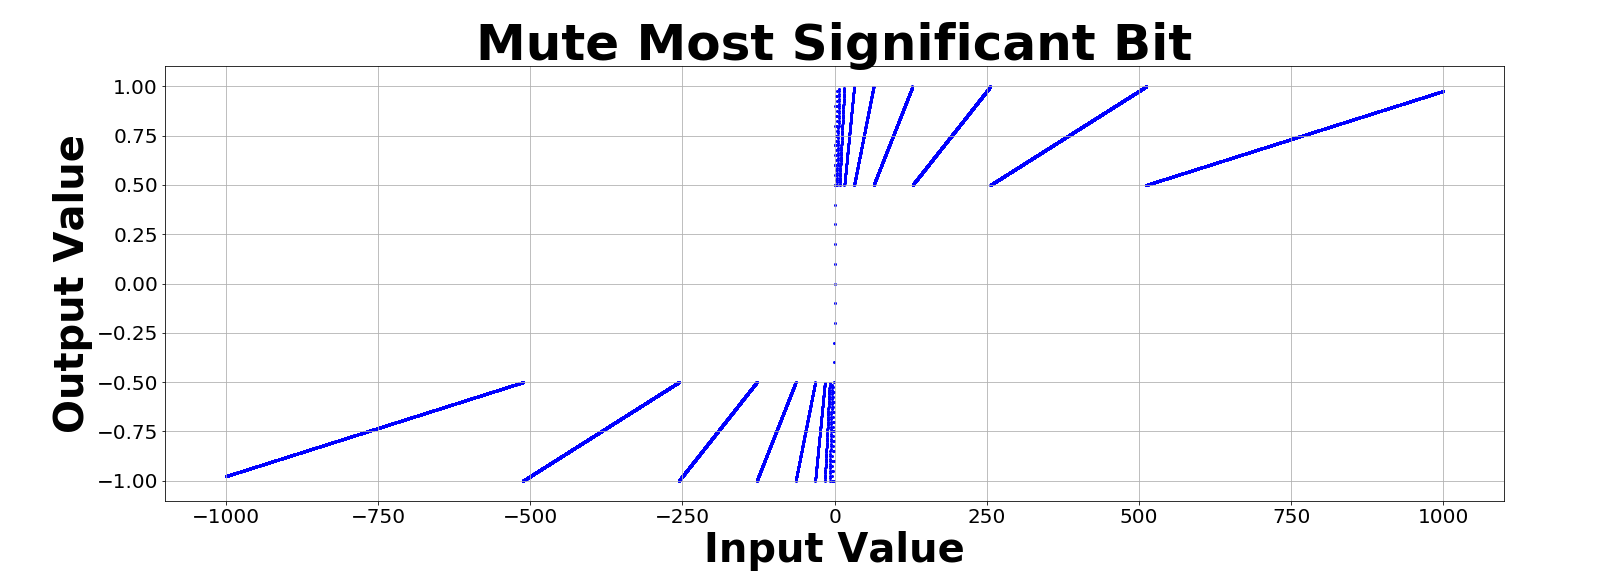
\includegraphics[width=0.3]{Mute_Most_Significant_Bit}
	\textcolor{red}{Please Help me with the formatting of this image!}
	\label{MUTE MSB}
	\caption{Input versus output values of float-ing point numbers subject to the \textit{mute most-significant-bit} attack function}
\end{figure}

\subsubsection{Experimental Setup}

\paragraph*{}The MLP neural network model is composed of multiple layers of \textit{neurons}, that each contain a real-valued floating-point number called an \textit{activation}.  In general, given a layer of activations $\vec{x}^{(l)}$ (The superscript is used as a layer index), the activations in the next sequential layer, $\vec{x}^{(l+1)}$, are produced with weighting matrix $\hat{W}^{(l)}$, bias vector $\vec{b}^{(l)}$, and activation function $f$ such that:

\begin{equation}
\label{feed-forward}
\vec{x}^{(l+1)} = f \Big( \hat{W}^{(l)} \vec{x}^{(l)} + \vec{b}^{(l)} \Big)
\end{equation}

The recurrence of equation (\ref{feed-forward}) is used to pass information forward through the network. In a network with $L$ layers, raw information is given with $\vec{x}^{(0)}$ and the network's prediction is given by the final layer, $\vec{x}^{(L-1)}$.

\paragraph*{}The Multilayer Perceptron network must then find a series of parameters, which are the elements in all weighting matrices and all bias vectors, that allows for a given sample to produce a low value for a given \textit{Loss function}. The loss function measures the difference between a networks given output and expected output; with better trained networks producing generally low loss values over a set of samples. The process of finding the values is called \textit{optimization}. There are many different algorithms that perform optimization, and for this experiment, we have chosen to use \textit{Stochastic Gradient Descent} (SGD) due to its widespread use and versatility. This method uses successive passes over a training data set to iterativly update model parameters such that they allow for a convergence is the lowest possible loss value.

\paragraph*{}To model a bit-muting attack, we introduce and \textit{attack function} that acts in the matrix-vector product 
in eqn. (\ref{feed-forward}). When a Boolean \textit{trigger condition} parameter is met, the MSB attack as described above, eqn. (\ref{feed-forward}) is instead replaced with it's attack variant:

\begin{equation}
\label{Attack}
\vec{x}^{(l+1)} = f \Big( A \big[ \hat{W}^{(l)} \vec{x}^{(l)} \big] + \vec{b}^{(l)} \Big)
\end{equation}

Where $A$ is the attack function, applied element-wise to each object in it's argument. 

\paragraph*{}For a practical demonstration of this attack function, we have tested it on variants of an image classification neural network. Each network was given of subset of training images from the MNIST data set, each containing a pixelized handwritten digit, labeled $0$ through $9$ according to the digit in that image. Each model was then trained on $6400$ similar, but non-identical images for evaluation. A subset of samples is visualized with a binary color map in fig. (\ref{MNIST})

\begin{figure}[h]
	\label{MNIST}
	\centering
	\textcolor{red}{Please Help me with the formatting of this image!}
	%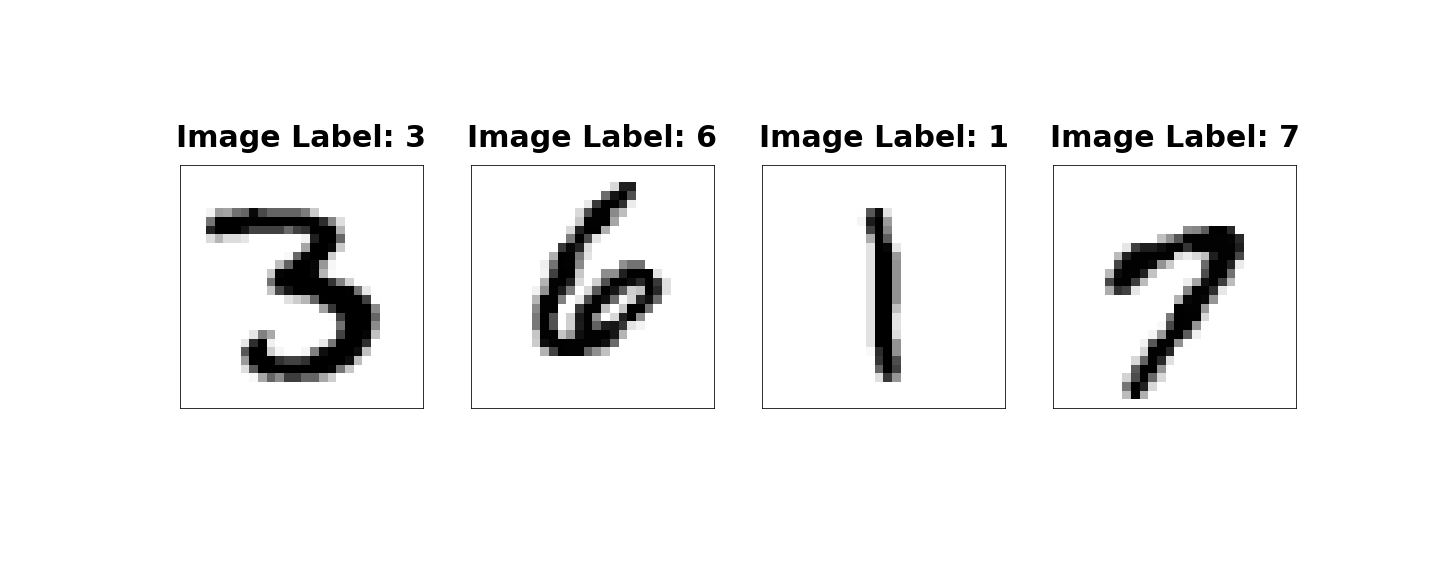
\includegraphics[scale=0.3]{MNIST}
	\caption{Four MNIST figures shaped as $28$ pixel by $28$ pixel images, colored with a binary color map along with their corresponding labels.}
\end{figure}

\paragraph*{}Each sample is $28 \times 28$ pixels, each containing by a single integer $0$ through $255$ (which are tranfomred into floats when passed through the network). Images were shaped shaped into a $784 \times 1$ array object and used as input into the network. This means for each network model, there are always $784$ input neurons and $10$ output neurons (one for each class). To test different model architecture complexities, we tested networks containing $1$, $2$, $3$, and $4$ hidden layers (referred to as \textit{network depth}) and used $20$, $40$, $60$, $80$, $100$, and $120$ neurons per layer (referred to as \textit{neuron density} or \textit{network width}). Permutations of these parameters allowed for us to record behavior over $24$ unique MLP model variants.

\subsubsection{Impact of Bit-Muting Attack Classification Metrics}

\paragraph*{}To measure the impact of this type of attack on the image classifier model, we test a baseline classifier against a classifier subject to a random 50/50 trigger condition. From each variant, we have recorded the following metrics:

\begin{enumerate}
\item \textbf{Accumulated loss function for the final iteration.} This value measures the difference between expected outcome of the network and the given outcome, with a generally lower value begin desirable.(Bounded to Positive Values). 
\item \textbf{Average precision score all 10 classes.} Precision score is the ratio of true positive selections to total sections. It measures how many selected items are relevant to the given task. (Bounded $[0,1]$, higher is favorable).
\item \textbf{Average recall score for all 10 classes.} Recall score is the ratio of true positive selections to relevant sections. It measures how many relevant items in the given task are selected. (Bounded $[0,1]$, higher is favorable).
\end{enumerate} 

\paragraph*{}In each of the 24 model variants (4 layer depths, 6 densities), 50 models were trained, with the average, minimum and maximum values for each of the four metrics noted. The average for each metric, across each model depth and neuron density is plotted in fig. (\ref{results}). Note that the lack of a data point means that the value of that metric diverged to infinity or some other undefined value.

\begin{figure}[h]
	\centering
	\textcolor{red}{Please Help me with the formatting of this image!}
	%\subfigure[]{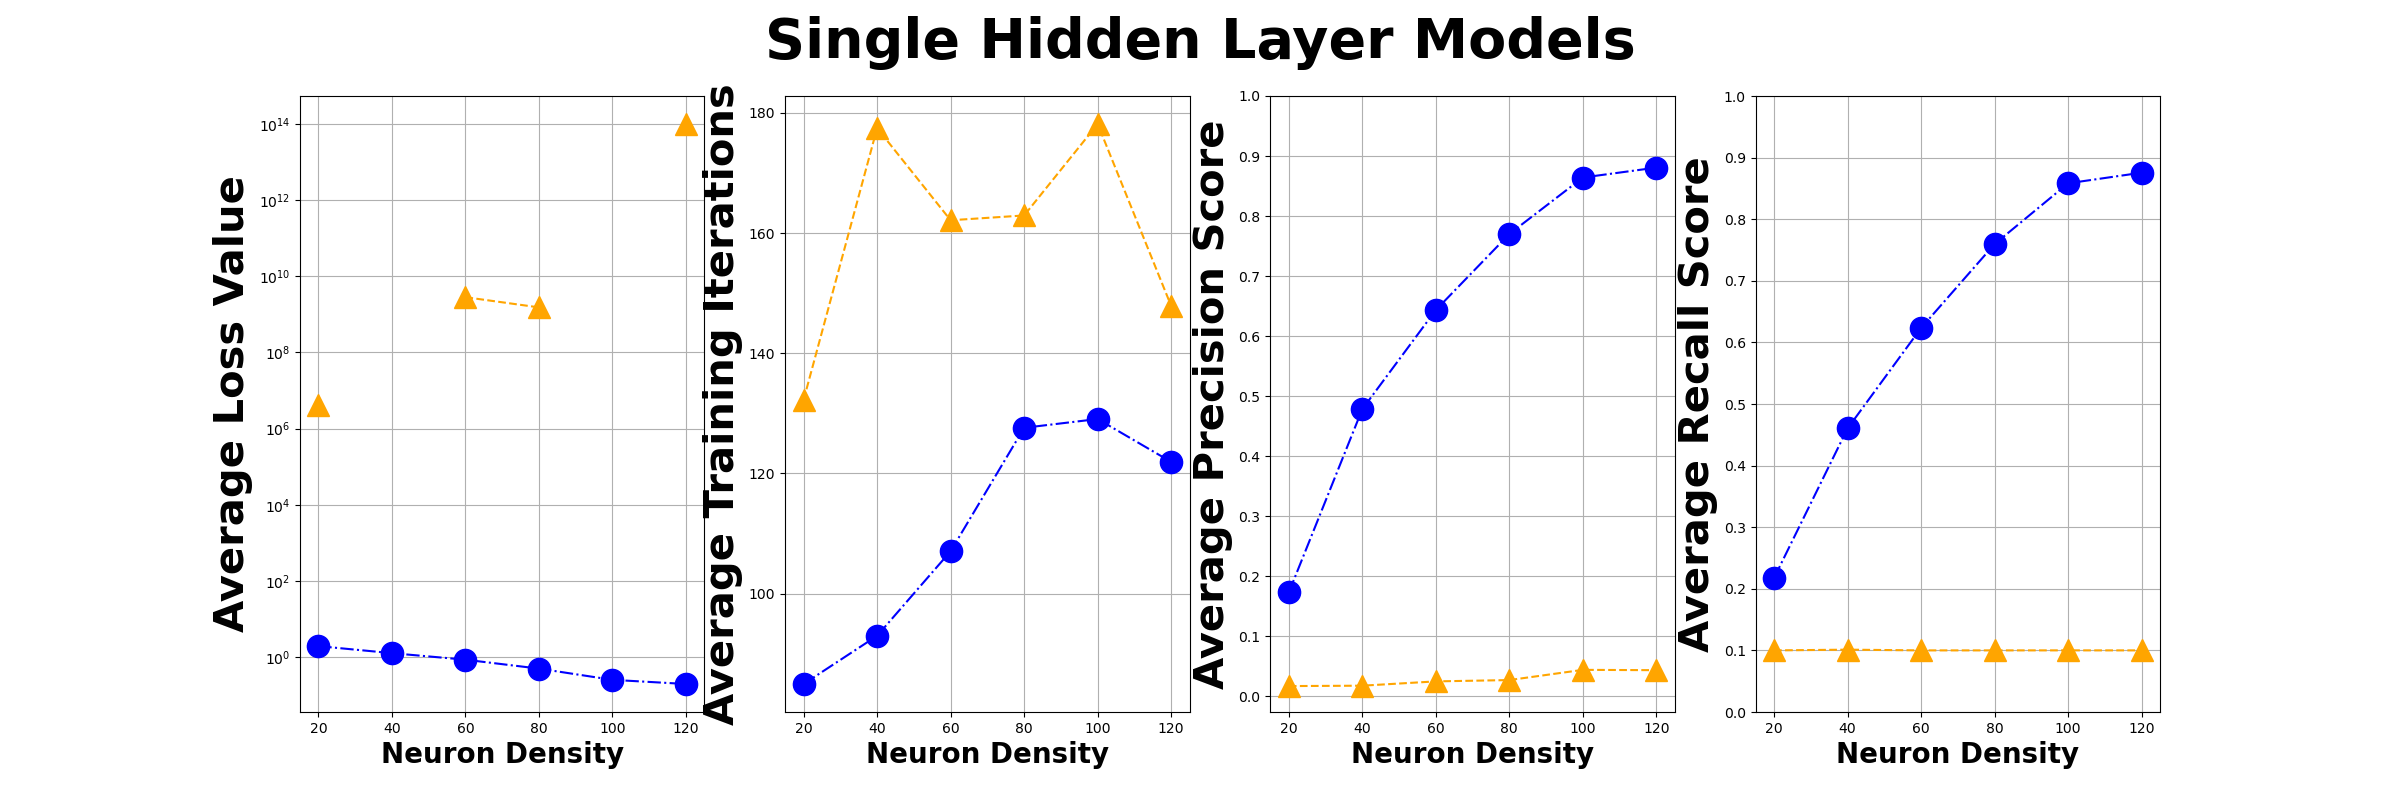
\includegraphics[scale=0.2]{Single_Hidden_Layer_Models}}
	%\subfigure[]{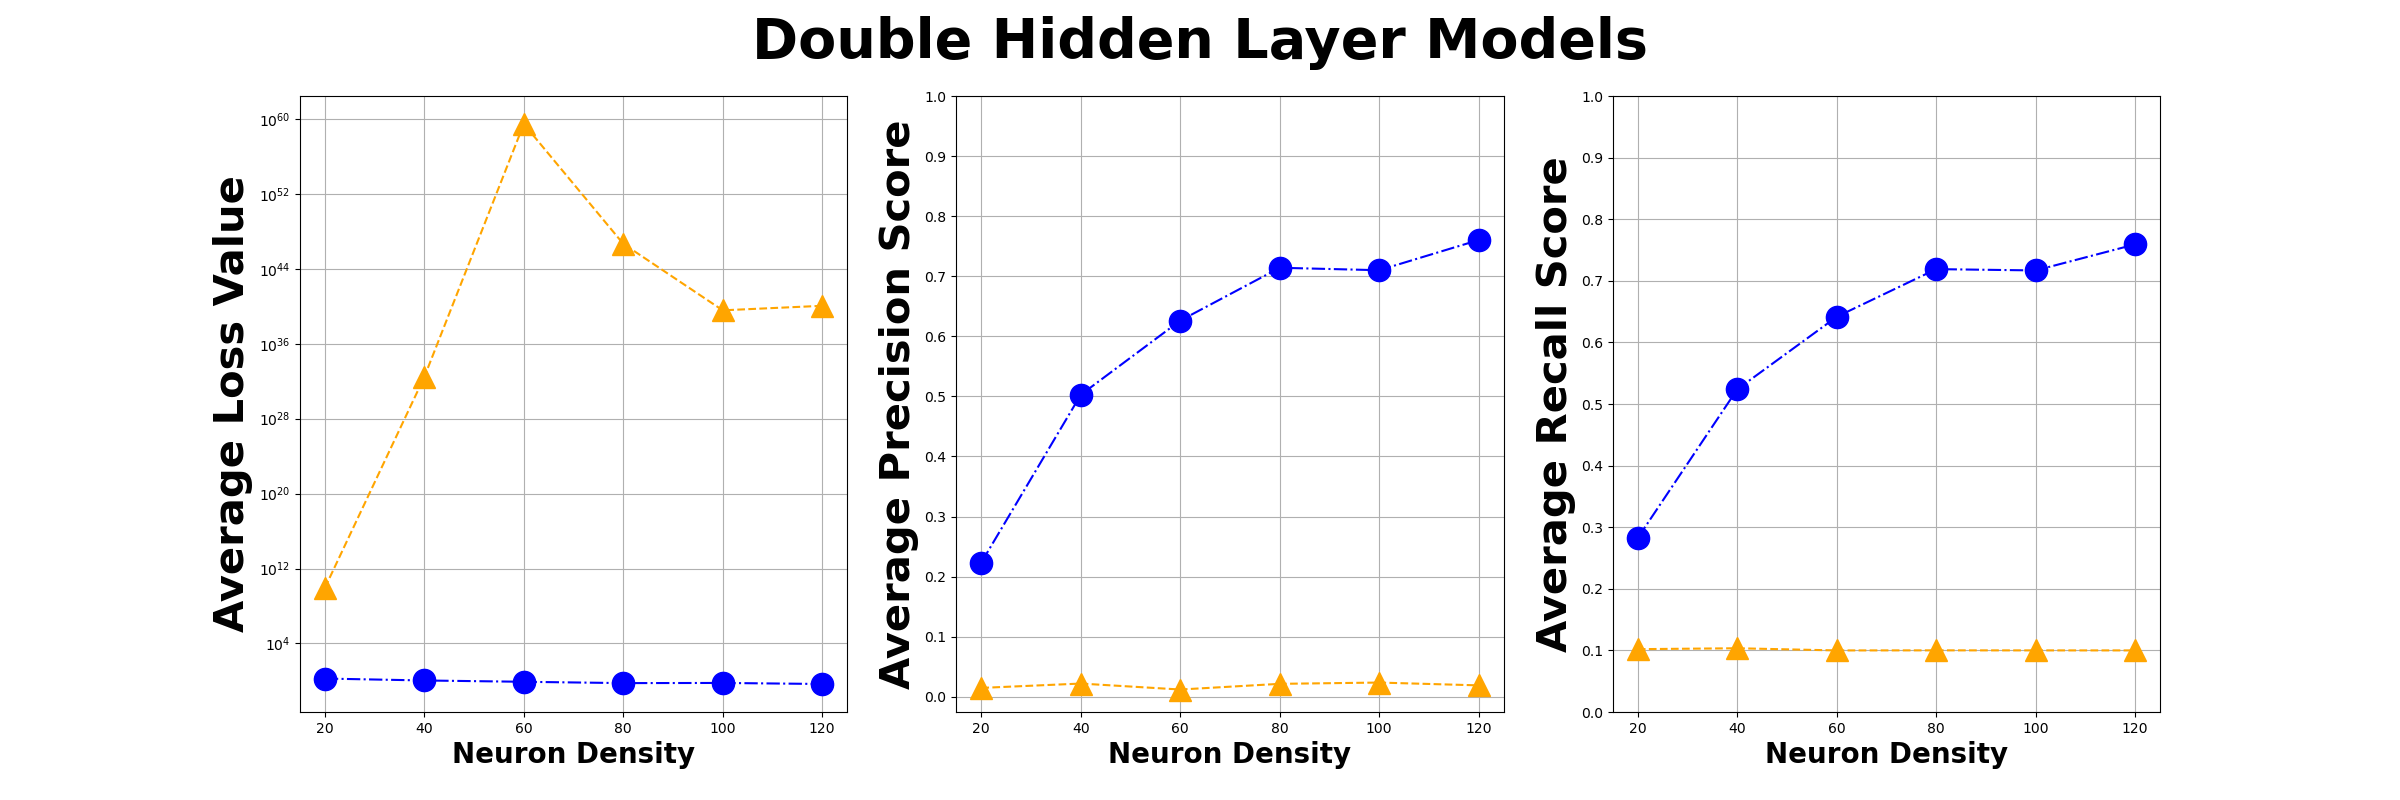
\includegraphics[scale=0.2]{Double_Hidden_Layer_Models}}
	%\subfigure[]{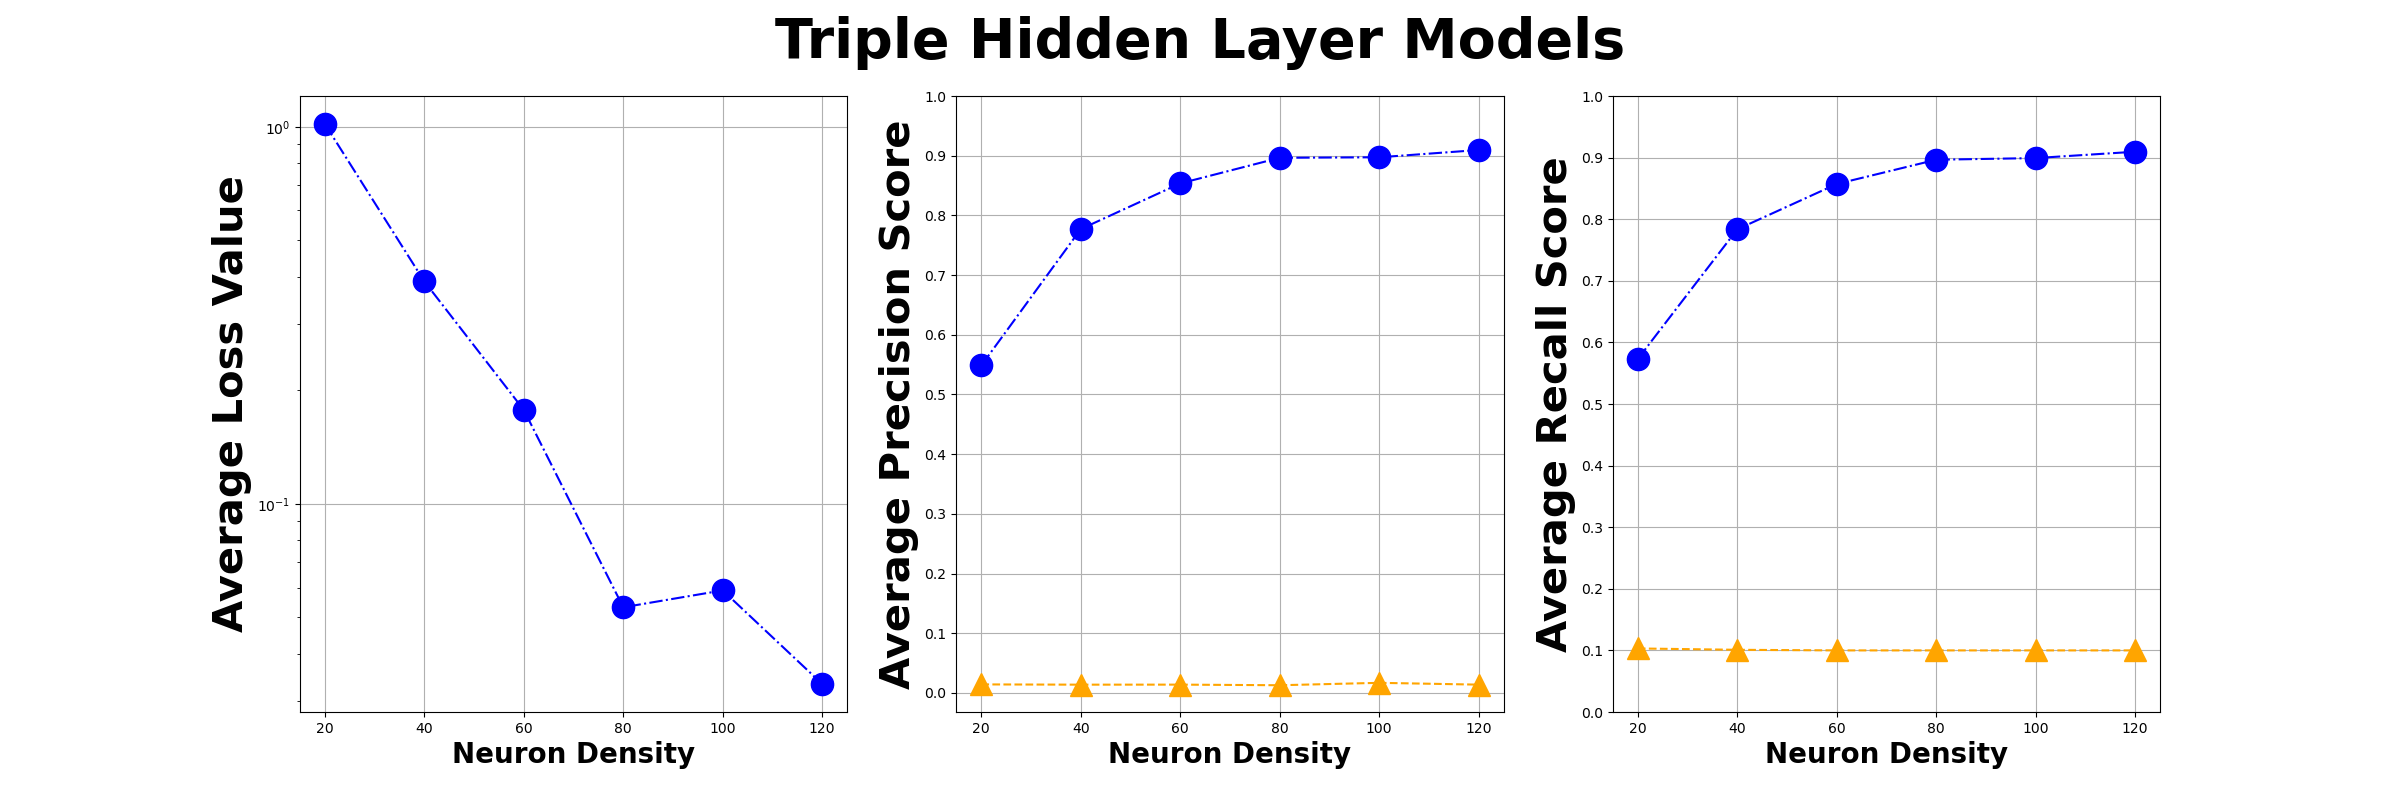
\includegraphics[scale=0.2]{Triple_Hidden_Layer_Models}}
	%\subfigure[]{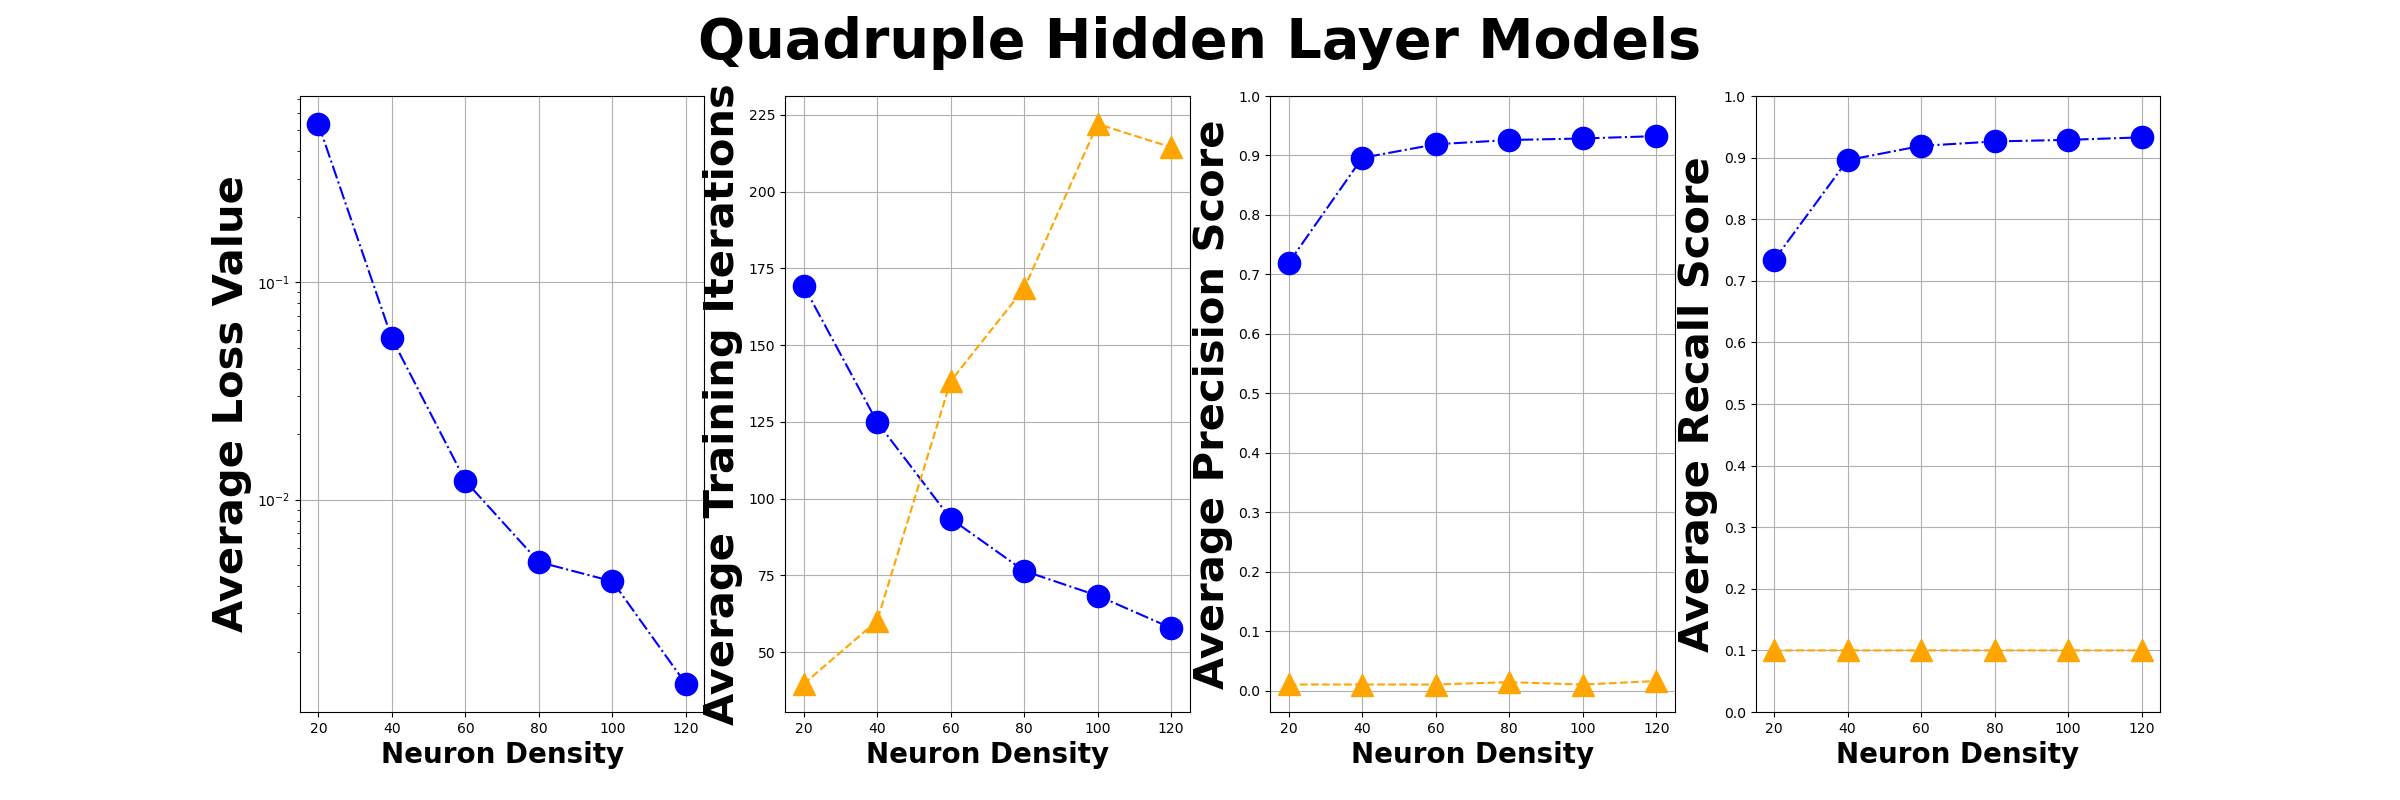
\includegraphics[scale=0.2]{Quadruple_Hidden_Layer_Models}}
	\label{results}
\end{figure}

\subsubsection{Conclusions from Bit-Muting Attack}

\paragraph*{}The application of a random bit-mute attack shows drastic difference in the final accumulated loss function value from the baseline model equivalent - plotted in the first column of each row. Results indicate that increasing model complexity leads to the baseline model showing progressively lower loss value, and thus a better fit. However, the corresponding attacked models produce loss values that diverge, and are often undefined Notice how for the 3 and 4 hidden layer models, all final loss function values are undefined. This occurs when the loss value exceeds the maximum value of a double-precision floating-point number and thus returns \textit{inf} or \textit{NaN}. 

\paragraph*{}Examining all model depths and all neuron densities, the baseline model shows a substantially higher precision and recall score than the corresponding attacked model. These differences are shown the two right-most subplots in each row. These classification metrics are commonly used together to quantify a network's ability to match samples with it's known target label in a validation set. 

\paragraph*{}These undefined values show that despite increasing complexity, the presence of the attack function prohibits the SGD optimizer from converging on a suitable set of parameters to fit the needed task. Despite the optimizer algorithm itself being unaffected, it is the replacement of eqn. (\ref{feed-forward}) with eqn. (\ref{Attack}) in select cases that prevents the network from making a proper decision in the first place. The SGD algorithm can only update the model based on the expected feed-forward mechanism, and thus can only correct for limited perturbations. These results show that a bit-muting algorithm creates devastating negative consequences and performance compromises across this given set of multilayer perceptron architectures.

% END LANDON'S ADDITIONS

\end{document}